\documentclass{beamer}
\usetheme{Darmstadt}
\definecolor{dgrey}{rgb}{0.25, 0.25, 0.25}
\usecolortheme[named=dgrey]{structure}

\usepackage[utf8]{inputenc}
\usepackage{graphicx}
\usepackage{multicol}
\usepackage{xcolor}

\definecolor{dgreen}{HTML}{005500}
\definecolor{dblue}{HTML}{000099}
\definecolor{dred}{HTML}{C00000}

\renewcommand{\.}{\hskip .75pt}

\DeclareMathOperator{\aand}{\;\wedge\;}
\DeclareMathOperator{\conv}{conv}

\newcommand\Wider[2][3em]{
	\makebox[\linewidth][c]{
		\begin{minipage}{\dimexpr\textwidth+#1\relax}
			\raggedright#2
		\end{minipage}
	}
}

\title{Computer Science Track Core Course}
\subtitle{Linear programming --- recitation 1}
\author{Martin Dvorak\\ISTA\\Kolmogorov group}
\date{2023-05-11}


\begin{document}


\begin{frame}
 	\titlepage
\end{frame}


\begin{frame}
	\frametitle{Linear program}
	\framesubtitle{Definitions}
	
	We are given an input $A \in \mathbb{Q}^{m \times n}$, $b \in \mathbb{Q}^{m}$, $c \in \mathbb{Q}^{n}$ and we search for $\bold{x} \in \mathbb{Q}^{n}$ that optimizes\.\dots
	\bigskip
	
	\begin{columns} 
		\begin{column}{0.5\textwidth}
		$$
		\begin{array}{lrcrcl}
			\text{minimize} & c'\. \bold{x} \\
			\text{s.\.t.} & A\. \bold{x} \ge b \\
		\end{array}
		$$
		\medskip
		
		$$
		\begin{array}{lrcrcl}
			\text{minimize} & c'\. \bold{x} \\
			\text{s.\.t.} & A\. \bold{x} = b \\
			\text{where} & \bold{x} \ge \bold{0}
		\end{array}
		$$
		\end{column}
		
		\begin{column}{0.5\textwidth}
		$$
		\begin{array}{lrcrcl}
			\text{maximize} & c'\. \bold{x} \\
			\text{s.\.t.} & A\. \bold{x} \le b \\
		\end{array}
		$$
		\medskip
		
		$$
		\begin{array}{lrcrcl}
			\text{maximize} & c'\. \bold{x} \\
			\text{s.\.t.} & A\. \bold{x} = b \\
			\text{where} & \bold{x} \ge \bold{0}
		\end{array}
		$$
		\end{column}
	\end{columns}
\end{frame}

\begin{frame}
	\frametitle{Example of LP}
	\framesubtitle{Separating points}
	We are searching for a line $y = ax + b$ that separates \textcolor{dgreen}{``disks'' (top)} from \textcolor{dblue}{``squares'' (bottom)}.
	
	\vspace*{-8pt}
	\hfil\hfil\hfil\hfil\hfil\hfil\hfil\hfil\hfil\hfil\hfil\hfil\hfil\hfil\hfil\hfil 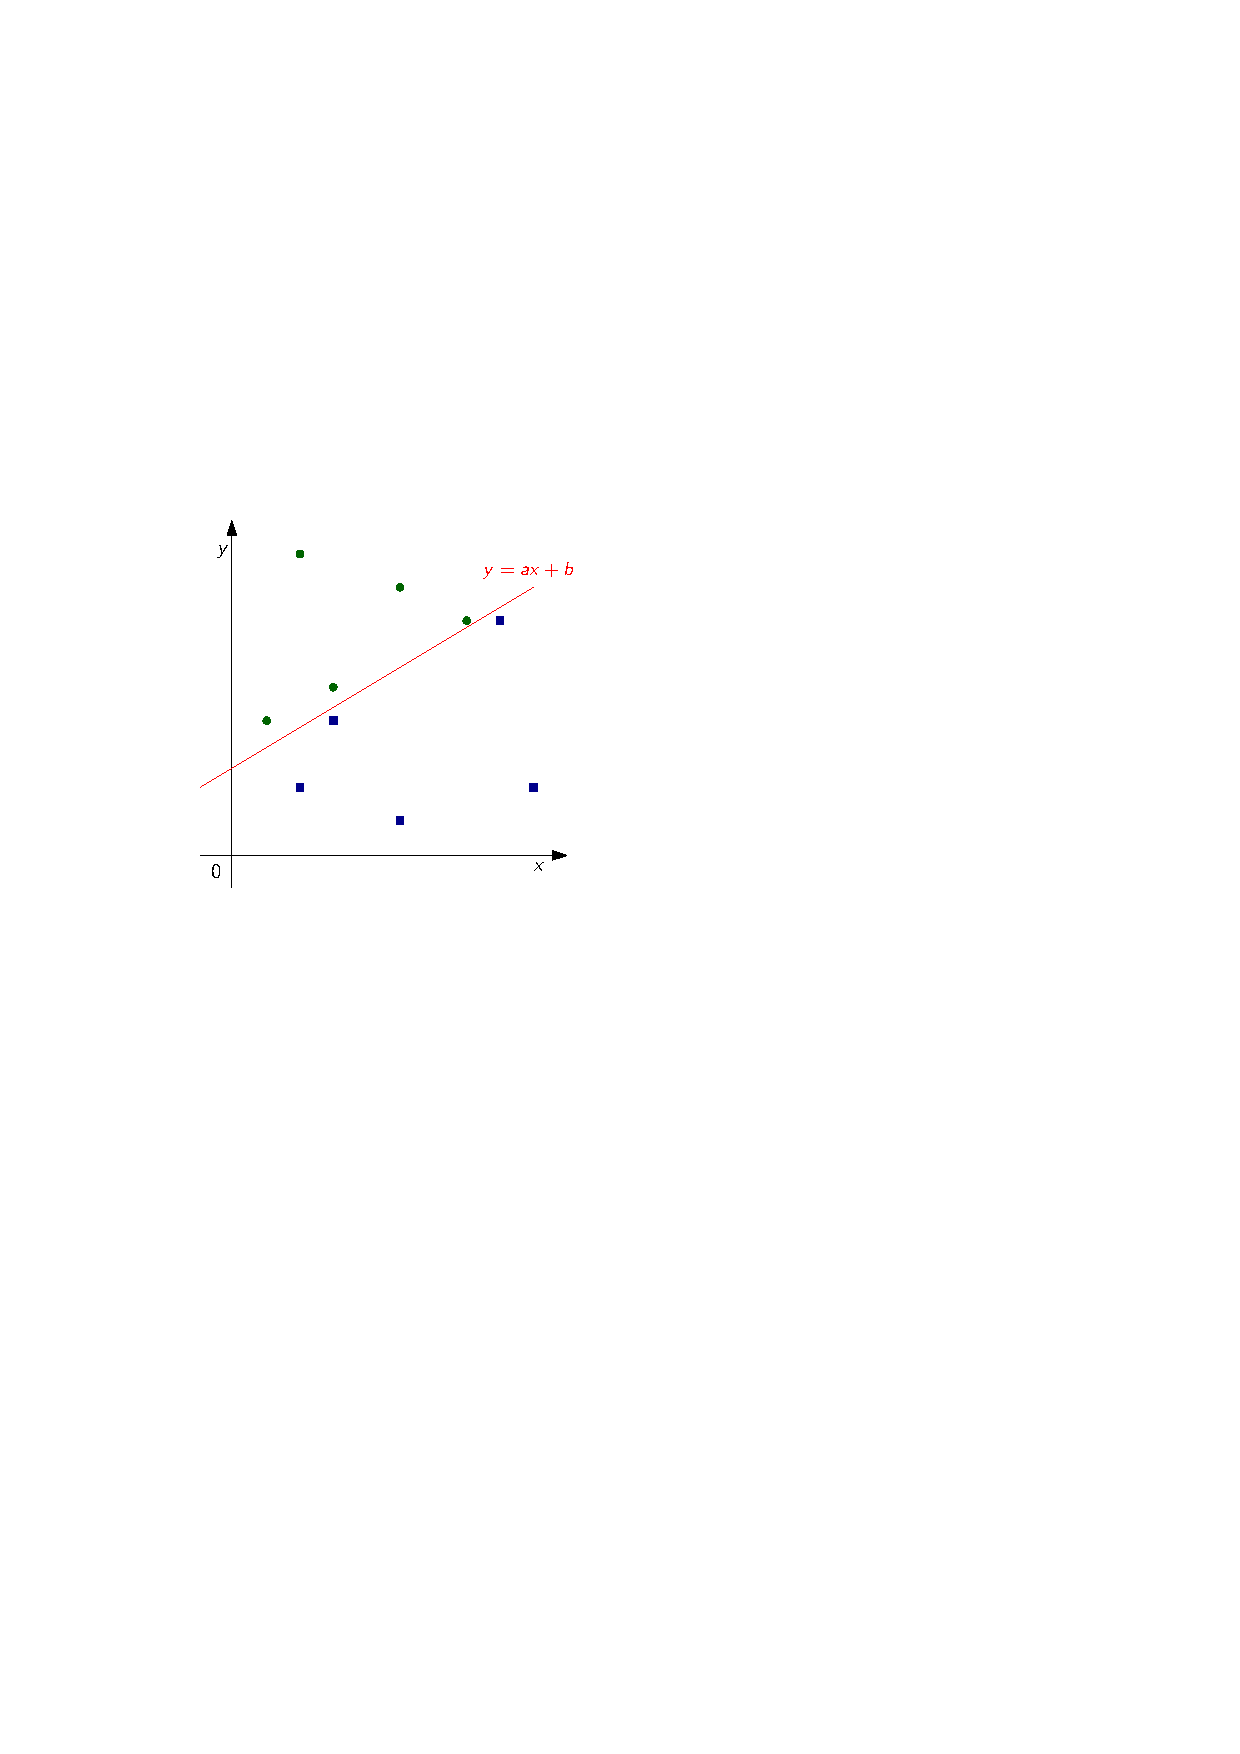
\includegraphics[width=0.44\textwidth]{separating}
	\vspace*{-8pt}
	
	\pause
	Variables: \pause $a \lessgtr 0$, $b \lessgtr 0$
	
	\pause
	Point $(x_1, y_1)$ above the line: \pause $x_1 \cdot a + b \le y_1$ ~~~ \textcolor{dgreen}{``disk''}
	
	\pause
	Point $(x_2, y_2)$ below the line: \pause $x_2 \cdot a + b \ge y_2$ ~~~ \textcolor{dblue}{``square''}
	
	\pause
	Objective: \pause minimize 0
\end{frame}

\begin{frame}
	\frametitle{Example of LP}
	\framesubtitle{Separating points strictly}
	Now, we are searching for a line $y = ax + b$ that separates them strictly.
	
	\vspace*{-8pt}
	\hfil\hfil\hfil\hfil\hfil\hfil\hfil\hfil\hfil\hfil\hfil\hfil\hfil\hfil\hfil\hfil 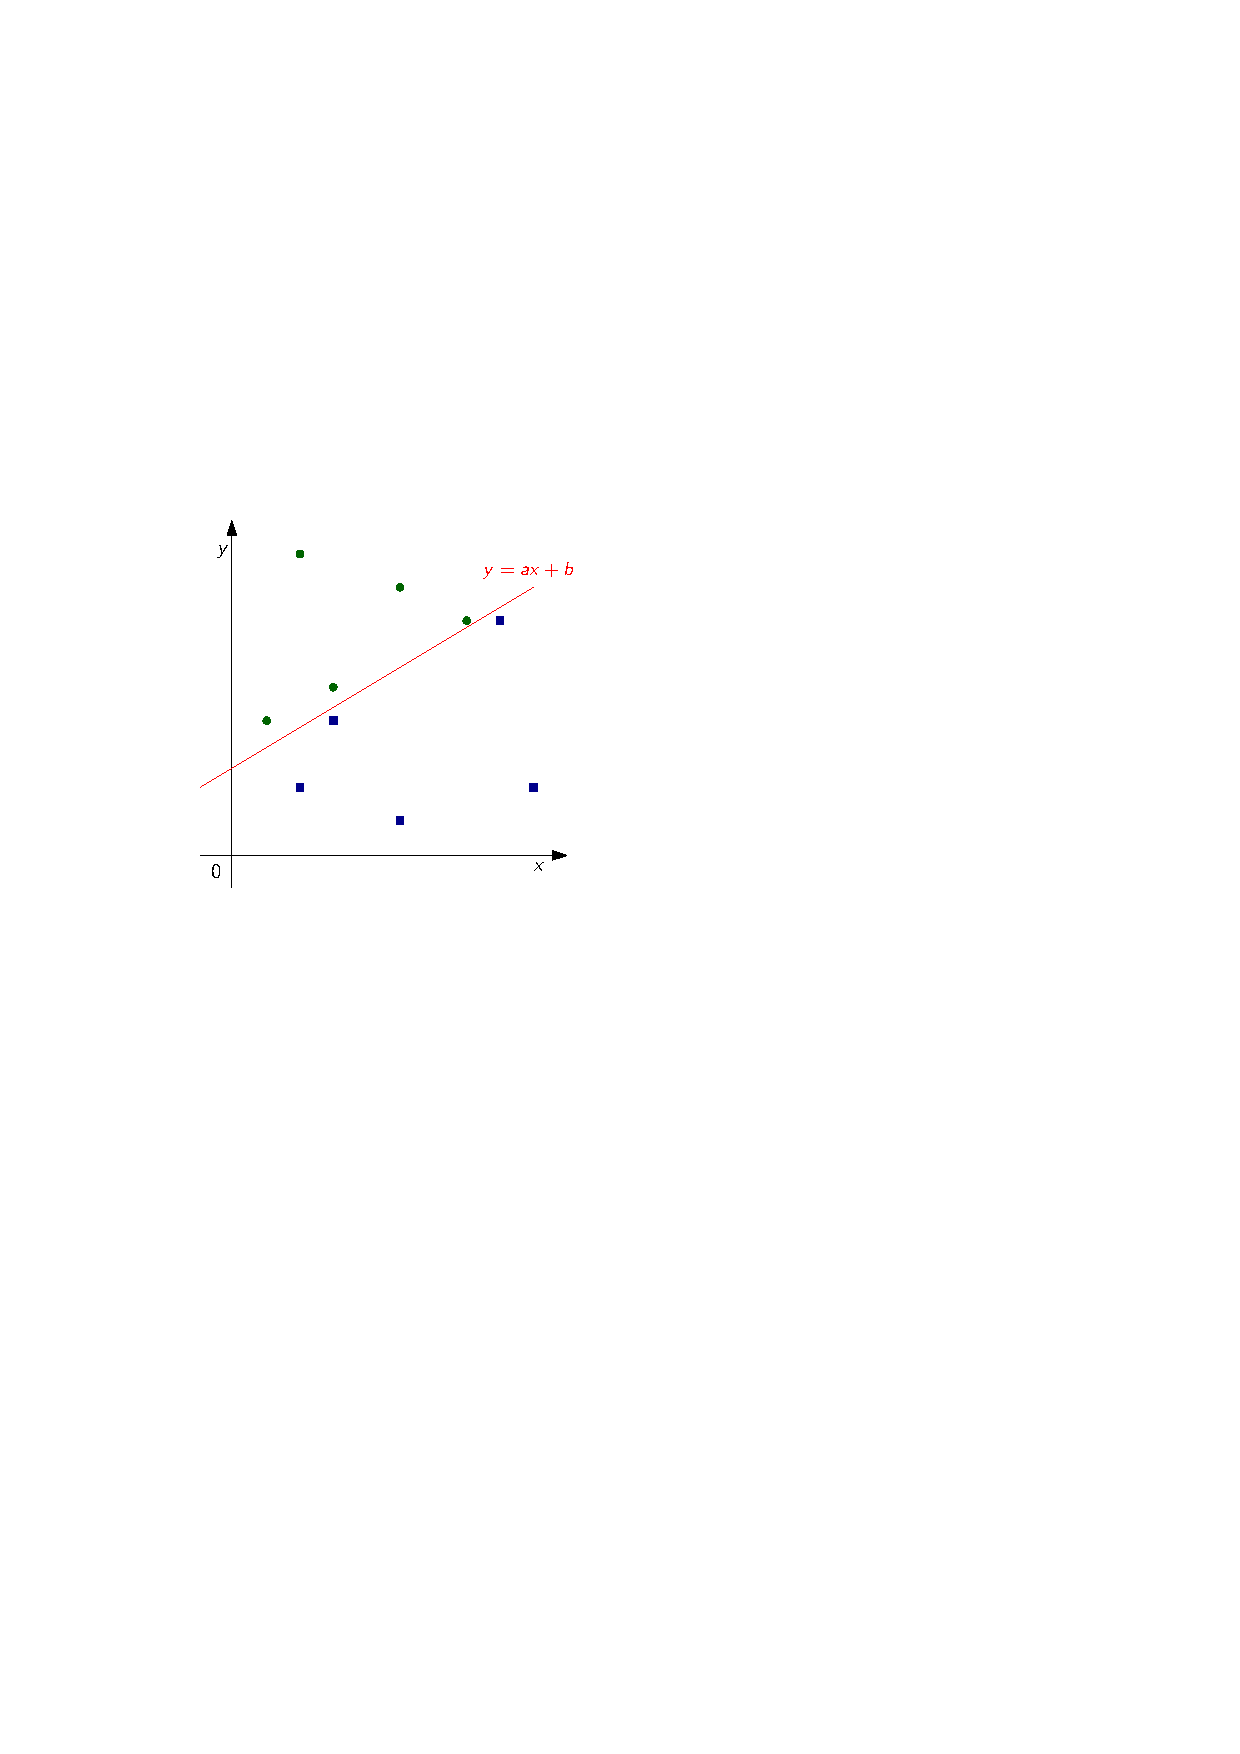
\includegraphics[width=0.44\textwidth]{separating}
	\vspace*{-8pt}
	
	\pause
	Variables: $a \lessgtr 0$, $b \lessgtr 0$, \textcolor{dred}{$d \ge 0$}
	
	Point $(x_1, y_1)$ above the line: $x_1 \cdot a + b ~\textcolor{dred}{+ \;d\;} \le y_1$
	
	Point $(x_2, y_2)$ below the line: $x_2 \cdot a + b ~\textcolor{dred}{- \;d\;} \ge y_2$
	
	Objective: maximize \textcolor{dred}{$d$}
\end{frame}

\begin{frame}
	\frametitle{Integer linear program}
	\framesubtitle{Definitions}
	
		We are given an input $A \in \mathbb{Z}^{m \times n}$, $b \in \mathbb{Z}^{m}$, $c \in \mathbb{Z}^{n}$ and we search for $\bold{x} \in \mathbb{Z}^{n}$ that optimizes\.\dots
	\bigskip
	
	\begin{columns} 
		\begin{column}{0.5\textwidth}
			$$
			\begin{array}{lrcrcl}
				\text{minimize} & c'\. \bold{x} \\
				\text{s.\.t.} & A\. \bold{x} \ge b \\
			\end{array}
			$$
			\medskip
			
			$$
			\begin{array}{lrcrcl}
				\text{minimize} & c'\. \bold{x} \\
				\text{s.\.t.} & A\. \bold{x} = b \\
				\text{where} & \bold{x} \ge \bold{0}
			\end{array}
			$$
		\end{column}
		
		\begin{column}{0.5\textwidth}
			$$
			\begin{array}{lrcrcl}
				\text{maximize} & c'\. \bold{x} \\
				\text{s.\.t.} & A\. \bold{x} \le b \\
			\end{array}
			$$
			\medskip
			
			$$
			\begin{array}{lrcrcl}
				\text{maximize} & c'\. \bold{x} \\
				\text{s.\.t.} & A\. \bold{x} = b \\
				\text{where} & \bold{x} \ge \bold{0}
			\end{array}
			$$
		\end{column}
	\end{columns}
\end{frame}

\begin{frame}
	\frametitle{Example of ILP}
	\framesubtitle{Separating points partially}
	
	\begin{columns}
		\begin{column}{0.5\textwidth}
			We are searching for a line $y = ax + b$ that separates given points --- \textcolor{dgreen}{``disks'' (top)} from \textcolor{dblue}{``squares'' (bottom)} --- with as few exceptions as possible.
			\medskip
			
			Let us ignore all vertical and nearly-vertical solutions.
			\medskip
			
			$M$ is a very large integer.
		\end{column}
	
		\begin{column}{0.5\textwidth}
			\begin{center}
				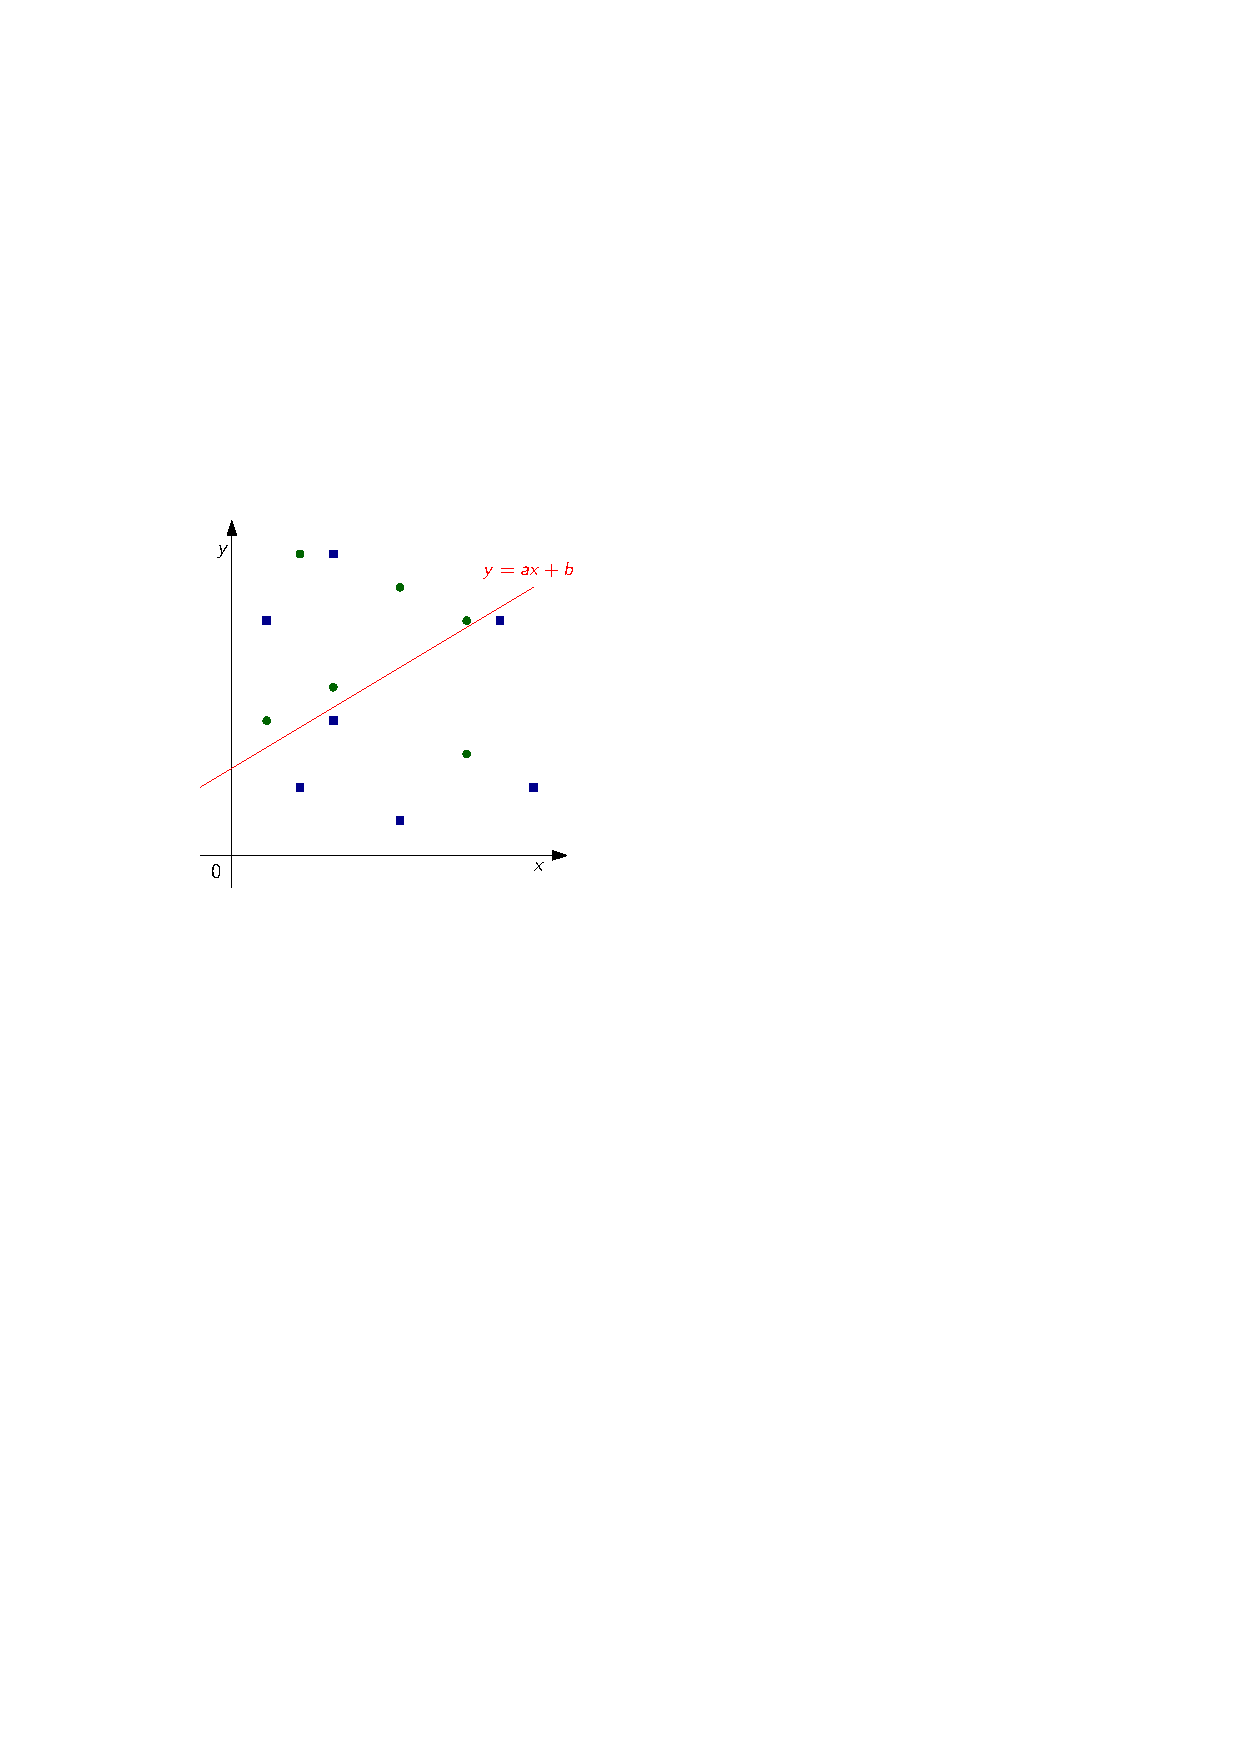
\includegraphics[width=0.88\textwidth]{separating_p}
			\end{center}
		\end{column}
	\end{columns}

	\Wider[6.6mm]{
		Variables: \pause $a \lessgtr 0$, $b \lessgtr 0$; $\,\forall i : \textcolor{dred}{p_i \in \{0,1\}}$

		\pause
		Point $(x_1, y_1)$ \textcolor{dgreen}{above} the line: 
		\pause $x_1 \cdot a + b \;\textcolor{dred}{- \,M \cdot p_i} \textcolor{dgreen}{\;\boldsymbol{\le}\;} y_1$ ~~~ \textcolor{dgreen}{``disk''}
		
		\pause
		Point $(x_2, y_2)$ \textcolor{dblue}{below} the line: 
		\pause $x_2 \cdot a + b \;\textcolor{dred}{+ \,M \cdot p_i} \textcolor{dblue}{\;\boldsymbol{\ge}\;} y_2$ ~~~ \textcolor{dblue}{``square''}
		
		\pause
		Objective: \pause minimize $\sum_i \textcolor{dred}{p_i}$
	}
\end{frame}

\begin{frame}
	\frametitle{Example of ILP}
	\framesubtitle{Separating points partially}	

	Variables: $a \lessgtr 0$, $b \lessgtr 0$; $\,\forall i : \textcolor{dred}{p_i \in \{0,1\}}$
	
	Point $(x_1, y_1)$ \textcolor{dgreen}{above} the line: 
	$x_1 \cdot a + b \;\textcolor{dred}{- \,M \cdot p_i} \textcolor{dgreen}{\;\boldsymbol{\le}\;} y_1$ ~~~ \textcolor{dgreen}{``disk''}
	
	Point $(x_2, y_2)$ \textcolor{dblue}{below} the line: 
	$x_2 \cdot a + b \;\textcolor{dred}{+ \,M \cdot p_i} \textcolor{dblue}{\;\boldsymbol{\ge}\;} y_2$ ~~~ \textcolor{dblue}{``square''}
		
	Objective: minimize $\sum_i \textcolor{dred}{p_i}$
	
	\begin{columns}
		\begin{column}{0.5\textwidth}
			\begin{center}
				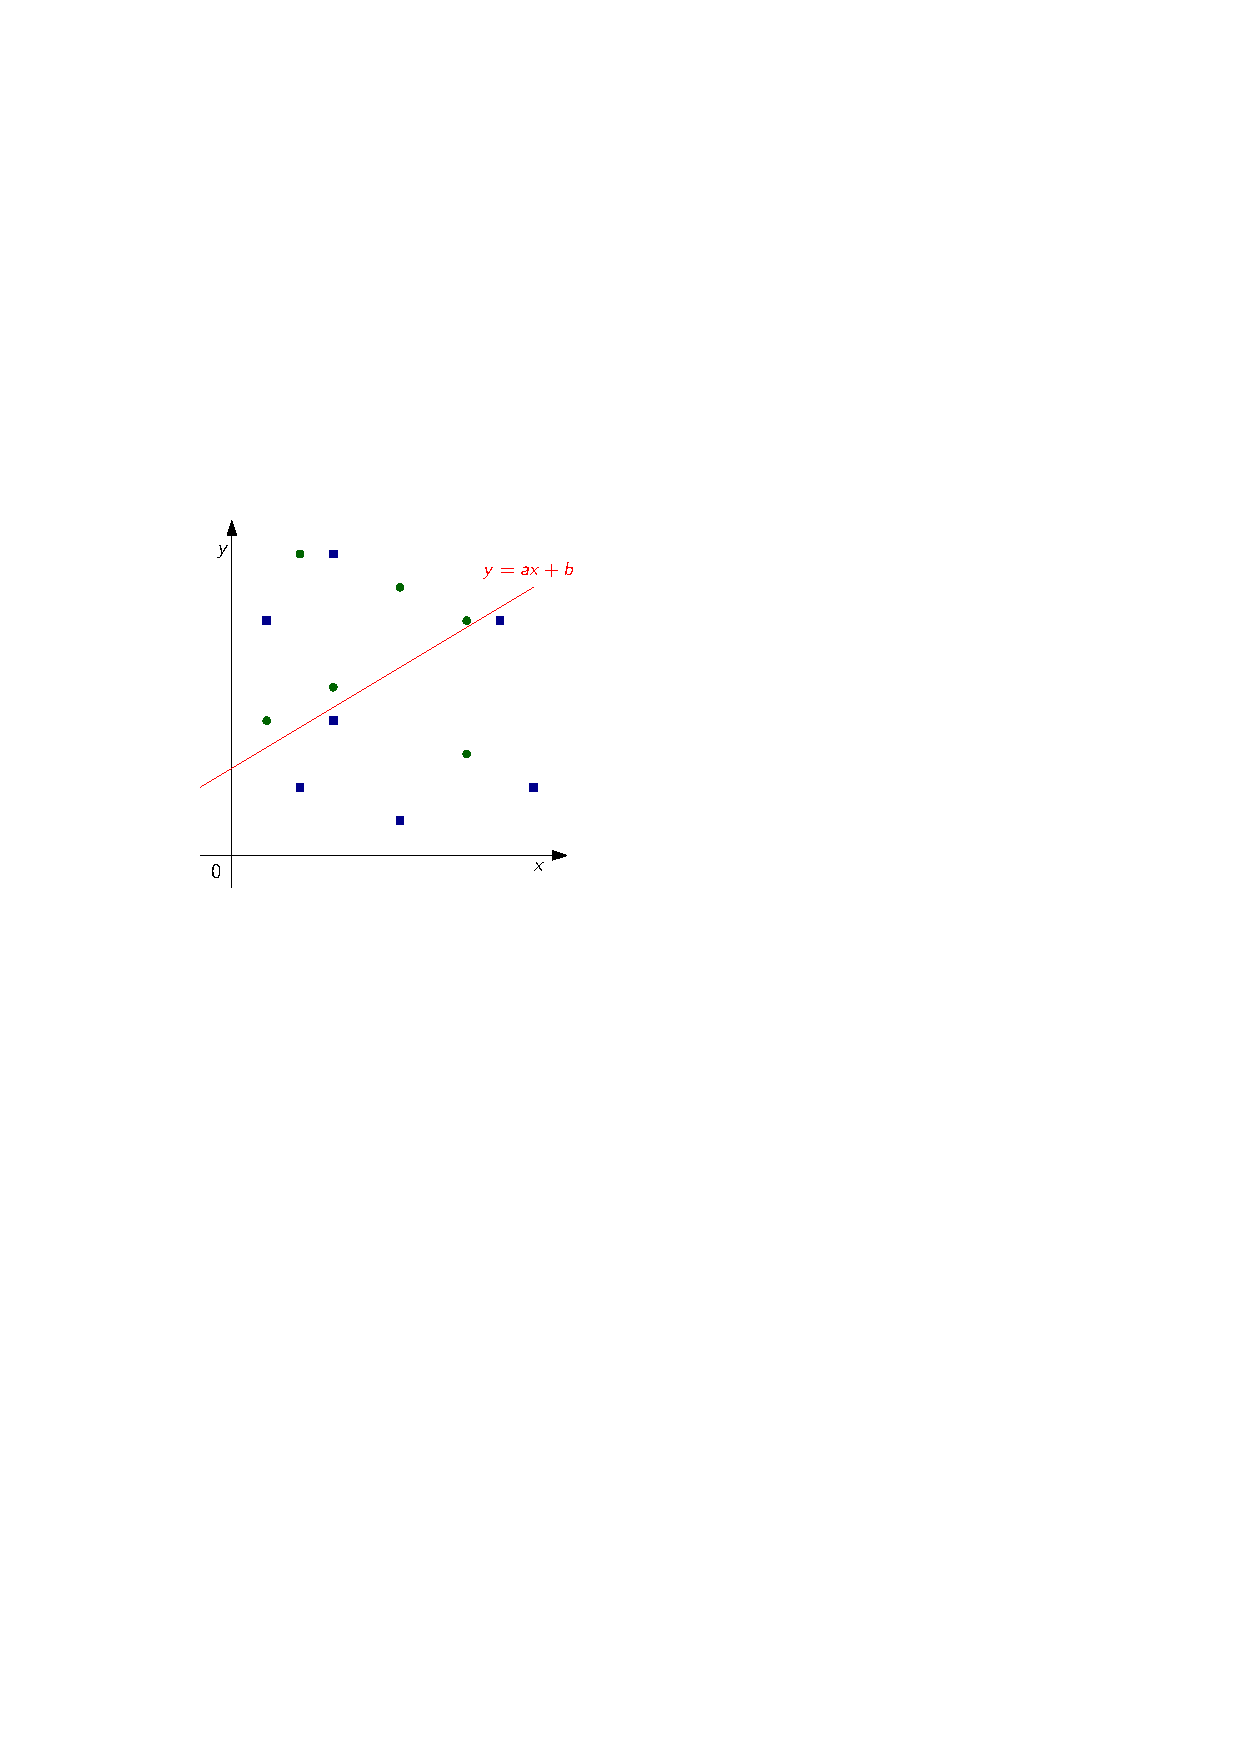
\includegraphics[width=0.88\textwidth]{separating_p}
			\end{center}
		\end{column}
	
		\begin{column}{0.5\textwidth}
			\pause Unfortunately, there is no general algorithm for solving ILP in polynomial time \pause (we don't know any such algorithm --- but most importantly, it cannot exist unless P = NP).
			\smallskip
			
			\pause This particular problem, however, can be solved in quadratic time.
			Consider all pairs of points.
		\end{column}
	\end{columns}
	
\end{frame}

\begin{frame}
	\frametitle{Example of LP duality}
	\framesubtitle{From minimization to maximization}
	
	Primal problem:
	$$
	\begin{array}{lrcrcl}
		\text{minimize\!\!\!\!} & \textcolor{dgreen}{6}x_1 & + & \textcolor{dgreen}{6}x_2 \\
		\text{s.\.t.} & 2x_1 & + & x_2 & \ge & \textcolor{dblue}{4} \\
		& x_1 & + & 2x_2 & \ge & \textcolor{dblue}{5} \\
		\text{where}& x_1, x_2 &\ge& 0~\,~ &
	\end{array}
	$$
	\pause 
	\bigskip
	
	Dual problem:
	$$
	\begin{array}{lrcrcl}
		\text{maximize\!\!\!\!} & \textcolor{dblue}{4}y_1 & + & \textcolor{dblue}{5}y_2 \\
		\text{s.\.t.} & 2y_1 & + & y_2 & \le & \textcolor{dgreen}{6} \\
		& y_1 & + & 2y_2 & \le & \textcolor{dgreen}{6} \\
		\text{where}& y_1, y_2 &\ge& 0~\,~ &
	\end{array}
	$$
	
\end{frame}

\begin{frame}
	\frametitle{Example of LP duality}
	\framesubtitle{From maximization to minimization}
	
	Dual problem:
	$$
	\begin{array}{lrcrcl}
		\text{maximize\!\!\!\!} & \textcolor{dblue}{4}y_1 & + & \textcolor{dblue}{5}y_2 \\
		\text{s.\.t.} & 2y_1 & + & y_2 & \le & \textcolor{dgreen}{6} \\
		& y_1 & + & 2y_2 & \le & \textcolor{dgreen}{6} \\
		\text{where}& y_1, y_2 &\ge& 0~\,~ &
	\end{array}
	$$
	\pause 
	\bigskip
	
	Dual of the dual problem:
	$$
	\begin{array}{lrcrcl}
		\text{minimize\!\!\!\!} & \textcolor{dgreen}{6}z_1 & + & \textcolor{dgreen}{6}z_2 \\
		\text{s.\.t.} & 2z_1 & + & z_2 & \ge & \textcolor{dblue}{4} \\
		& z_1 & + & 2z_2 & \ge & \textcolor{dblue}{5} \\
		\text{where}& z_1, z_2 &\ge& 0~\,~ &
	\end{array}
	$$
	
\end{frame}

\begin{frame}
	\frametitle{Example of LP duality}
	\framesubtitle{Comparison}
	
	Primal problem:
	$$
	\begin{array}{lrcrcl}
		\text{minimize\!\!\!\!} & \textcolor{dgreen}{6}x_1 & + & \textcolor{dgreen}{6}x_2 \\
		\text{s.\.t.} & 2x_1 & + & x_2 & \ge & \textcolor{dblue}{4} \\
		& x_1 & + & 2x_2 & \ge & \textcolor{dblue}{5} \\
		\text{where}& x_1, x_2 &\ge& 0~\,~ &
	\end{array}
	$$
	\bigskip
	
	Dual of the dual problem:
	$$
	\begin{array}{lrcrcl}
		\text{minimize\!\!\!\!} & \textcolor{dgreen}{6}z_1 & + & \textcolor{dgreen}{6}z_2 \\
		\text{s.\.t.} & 2z_1 & + & z_2 & \ge & \textcolor{dblue}{4} \\
		& z_1 & + & 2z_2 & \ge & \textcolor{dblue}{5} \\
		\text{where}& z_1, z_2 &\ge& 0~\,~ &
	\end{array}
	$$
	
\end{frame}


\begin{frame}
	\frametitle{LP duality}
	\framesubtitle{In general (I)}
	
	We are given $A \in \mathbb{Q}^{m \times n}$, $\textcolor{dblue}{b} \in \mathbb{Q}^{m}$,
    $\textcolor{dgreen}{c} \in \mathbb{Q}^{n}$ on the input.	
	
	We search for either $\bold{x} \in \mathbb{Q}^{n}$ or $\bold{y} \in \mathbb{Q}^{m}$.
	\bigskip
	
	Primal problem:
	$$
	\begin{array}{lrcrcl}
		\text{minimize} & \textcolor{dgreen}{c}'\. \bold{x} \\
		\text{s.\.t.} & A\. \bold{x} \ge \textcolor{dblue}{b} \\
		\text{where} & \bold{x} \;\textcolor{dred}{\lessgtr}\; \bold{0}
	\end{array}
	$$		
	\smallskip
	
	Dual problem:
	$$
	\begin{array}{lrcrcl}
		\text{maximize} & \textcolor{dblue}{b}'\. \bold{y} \\
		\text{s.\.t.} & A^{\!\top} \bold{y} \;\textcolor{dred}{=}\; \textcolor{dgreen}{c} \\
		\text{where} & \bold{y} \ge \bold{0}
	\end{array}
	$$	
\end{frame}

\begin{frame}
\frametitle{LP duality}
\framesubtitle{In general (II)}

	We are given $A \in \mathbb{Q}^{m \times n}$, $\textcolor{dblue}{b} \in \mathbb{Q}^{m}$, $\textcolor{dgreen}{c} \in \mathbb{Q}^{n}$ on the input.	
	
	We search for either $\bold{x} \in \mathbb{Q}^{n}$ or $\bold{y} \in \mathbb{Q}^{m}$.
	\bigskip
	
	Primal problem:
	$$
	\begin{array}{lrcrcl}
		\text{minimize} & \textcolor{dgreen}{c}'\. \bold{x} \\
		\text{s.\.t.} & A\. \bold{x} = \textcolor{dblue}{b} \\
		\text{where} & \bold{x} \;\textcolor{dred}{\ge}\; \bold{0}
	\end{array}
	$$		
	\smallskip
	
	Dual problem:
	$$
	\begin{array}{lrcrcl}
		\text{maximize} & \textcolor{dblue}{b}'\. \bold{y} \\
		\text{s.\.t.} & A^{\!\top} \bold{y} \;\textcolor{dred}{\le}\; \textcolor{dgreen}{c} \\
		\text{where} & \bold{y} \lessgtr \bold{0}
	\end{array}
	$$

\end{frame}

\begin{frame}
	\frametitle{LP duality}
	\framesubtitle{In general (III)}
	
	We are given $A \in \mathbb{Q}^{m \times n}$, $\textcolor{dblue}{b} \in \mathbb{Q}^{m}$, $\textcolor{dgreen}{c} \in \mathbb{Q}^{n}$ on the input.	
	
	We search for either $\bold{x} \in \mathbb{Q}^{n}$ or $\bold{y} \in \mathbb{Q}^{m}$.
	\bigskip
	
	Primal problem:
	$$
	\begin{array}{lrcrcl}
		\text{minimize} & \textcolor{dgreen}{c}'\. \bold{x} \\
		\text{s.\.t.} & A\. \bold{x} \ge \textcolor{dblue}{b} \\
		\text{where} & \bold{x} \;\textcolor{dred}{\ge}\; \bold{0}
	\end{array}
	$$		
	\smallskip
	
	Dual problem:
	$$
	\begin{array}{lrcrcl}
		\text{maximize} & \textcolor{dblue}{b}'\. \bold{y} \\
		\text{s.\.t.} & A^{\!\top} \bold{y} \;\textcolor{dred}{\le}\; \textcolor{dgreen}{c} \\
		\text{where} & \bold{y} \ge \bold{0}
	\end{array}
	$$

\end{frame}



\begin{frame}
	\frametitle{Combinations of vectors (linear, affine, convex)}
	\framesubtitle{Definition}
	
	Let $V$ be a vector space over $F$.		
	Consider vectors $\bold{x_1}, \dots, \bold{x_n} \in V$.
	\smallskip
	
	\begin{itemize}
		\setlength{\abovedisplayskip}{0pt}
		\setlength{\belowdisplayskip}{4pt}
		\pause \item We say that $\bold{y} \in\! V$ is a \textcolor{dred}{linear combination} of $\bold{x_1}, \dots, \bold{x_n}$ if:
		$$\exists\, \alpha_i, \dots, \alpha_n \in F : \ \  \textcolor{dgreen}{\sum_{i=1}^{n} \alpha_i \bold{x_i} = \bold{y}}$$
		\pause \item We say that $\bold{y} \in\! V$ is an \textcolor{dred}{affine combination} of $\bold{x_1}, \dots, \bold{x_n}$ if:
		$$\exists\, \alpha_i, \dots, \alpha_n \in F : \ \   \textcolor{dblue}{\sum_{i=1}^{n} \alpha_i = 1} \aand \textcolor{dgreen}{\sum_{i=1}^{n} \alpha_i \bold{x_i} = \bold{y}}$$
		\pause \item Suppose now that $F$ is a totally ordered field.
		
		Denote the set of $\varphi \in\! F$ such that $\varphi \textcolor{dblue}{\:\ge 0}$ by the symbol \textcolor{dblue}{$F_0^+$}.
		
		We say that $\bold{y} \in\! V$ is a \textcolor{dred}{convex combination} of $\bold{x_1}, \dots, \bold{x_n}$ if:
		$$\exists\, \alpha_i, \dots, \alpha_n \in \textcolor{dblue}{F_0^+} : \ \   \textcolor{dblue}{\sum_{i=1}^{n} \alpha_i = 1} \aand \textcolor{dgreen}{\sum_{i=1}^{n} \alpha_i \bold{x_i} = \bold{y}}$$
	\end{itemize}
\end{frame}

\begin{frame}
	\frametitle{Combinations of vectors (linear, affine, convex)}
	\framesubtitle{Quiz}
	
	Let $d \in \mathbb{Z}$ such that $d \ge 2$. 
	
	What is the \textcolor{dblue}{maximum} possible amount (largest set) of:
	\begin{itemize}
		\item \textcolor{dred}{Linear}ly independent vectors in $\mathbb{Z}_2^d$ over $\mathbb{Z}_2\,$? \\
		\visible<2->{\textcolor{dblue}{$d$}}
		\item \textcolor{dred}{Affine}ly independent vectors in $\mathbb{C}^d$ over $\mathbb{C}\,$? \\
		\visible<3->{\textcolor{dblue}{$d+1$}}
		\item \textcolor{dred}{Convex}ly independent vectors in $\mathbb{Q}^d$ over $\mathbb{Q}\,$? \\
		\visible<4->{\textcolor{dblue}{$\infty$}}
	\end{itemize}

\end{frame}

\begin{frame}
	\frametitle{Combinations of vectors (linear, affine, convex)}
	\framesubtitle{Basic properties}
	
	
	$\{ \text{\textcolor{dred}{convex combin.}} \} \;\subseteq\; \{ \text{\textcolor{dred}{affine combin.}} \} \;\subseteq\; \{ \text{\textcolor{dred}{linear combin.}} \}$
	
	\bigskip
	
	\pause Let \textcolor{dblue}{$V$} be a \textcolor{dblue}{vector space} and \textcolor{dblue}{$X \subseteq V$}.
	\begin{itemize}
		\item \textcolor{dblue}{$X$} is \textcolor{dred}{convex}ly \textcolor{dblue}{dependent}. $\implies$ 
		\textcolor{dblue}{$X$} is \textcolor{dred}{affine}ly \textcolor{dblue}{dependent}. \\ $\implies$
		\textcolor{dblue}{$X$} is \textcolor{dred}{linear}ly \textcolor{dblue}{dependent}.
		
		\item \textcolor{dblue}{$X$} is \textcolor{dred}{linear}ly \textcolor{dblue}{independent}. $\implies$ 
		\textcolor{dblue}{$X$} is \textcolor{dred}{affine}ly \textcolor{dblue}{independent}. \\ $\implies$
		\textcolor{dblue}{$X$} is \textcolor{dred}{convex}ly \textcolor{dblue}{independent}.
	\end{itemize}	
	\medskip

	\pause Let us have a \textcolor{dgreen}{matrix $A \in F^{m \times n}$} and a \textcolor{dgreen}{vector $b \in F^m$}.\\ We search for a \textcolor{dgreen}{solution $x \in F^n$}.
	\begin{itemize}
		\item \textcolor{dgreen}{$Ax = 0$} : Any \textcolor{dred}{linear combination} of \textcolor{dgreen}{solutions} is a \textcolor{dgreen}{solution}.
		\item \textcolor{dgreen}{$Ax = b$} : Any \textcolor{dred}{affine combination} of \textcolor{dgreen}{solutions} is a \textcolor{dgreen}{solution}.
		\item \textcolor{dgreen}{$Ax \le b$} : Any \textcolor{dred}{convex combination} of \textcolor{dgreen}{solutions} is a \textcolor{dgreen}{solution}.\\
		In this example, \textcolor{dgreen}{$F$} must be a totally ordered field.
	\end{itemize}
	
\end{frame}


\end{document}